% document type
\documentclass [12pt,oneside,a4]{report} % oneside
%\documentclass [12pt,twoside,openright,a4]{report} % twosided

% fixes
\usepackage{fixltx2e} % LaTeX patches, \textsubscript
\usepackage{cmap} % fix search and cut-and-paste in PDF

% language
\usepackage[english]{babel}
\usepackage[T1]{fontenc}
\usepackage[utf8]{inputenc}

% usability
\usepackage {makeidx}
\usepackage {float}
\usepackage {afterpage}
\usepackage {etoolbox}

% formatting
\usepackage{amsmath}
\usepackage{url}
\usepackage{setspace}
\usepackage{hyperref}

\usepackage{verbatim}
\usepackage{fancyvrb}
\usepackage{mdwlist}
\usepackage{float,caption}

\usepackage{tikz}
\usetikzlibrary{fit, positioning, arrows, backgrounds, shapes}

\usepackage{algorithm}
\usepackage{algorithmicx}
\usepackage[noend]{algpseudocode}

\usepackage{graphicx}
\usepackage{ifpdf}
\usepackage{listings, textcomp, color, xcolor, caption}

\usepackage{dirtree}

\usepackage{todonotes}

\makeindex

% Defines a `datastore' shape for use in DFDs.  This inherits from a
% rectangle and only draws two horizontal lines.
\makeatletter
\pgfdeclareshape{datastore}{
	\inheritsavedanchors[from=rectangle]
	\inheritanchorborder[from=rectangle]
	\inheritanchor[from=rectangle]{center}
	\inheritanchor[from=rectangle]{base}
	\inheritanchor[from=rectangle]{north}
	\inheritanchor[from=rectangle]{north east}
	\inheritanchor[from=rectangle]{east}
	\inheritanchor[from=rectangle]{south east}
	\inheritanchor[from=rectangle]{south}
	\inheritanchor[from=rectangle]{south west}
	\inheritanchor[from=rectangle]{west}
	\inheritanchor[from=rectangle]{north west}
	\backgroundpath{
	%  store lower right in xa/ya and upper right in xb/yb
		\southwest \pgf@xa=\pgf@x \pgf@ya=\pgf@y
		\northeast \pgf@xb=\pgf@x \pgf@yb=\pgf@y
		\pgfpathmoveto{\pgfpoint{\pgf@xa}{\pgf@ya}}
		\pgfpathlineto{\pgfpoint{\pgf@xb}{\pgf@ya}}
		\pgfpathmoveto{\pgfpoint{\pgf@xa}{\pgf@yb}}
		\pgfpathlineto{\pgfpoint{\pgf@xb}{\pgf@yb}}
	}
}

\tikzset{%
	pool/.style={%
		datastore,
		draw, very thick, fill=white, 
		minimum height=3em, minimum width=3em, 
		node distance=9em, font={\sffamily\bfseries}
	},
	process/.style={%
		draw, very thick, fill=white, 
		circle,
		minimum height=2em, minimum width=4em,
		node distance=9em, font={\sffamily\bfseries}
	},
	dataset/.style={%
		draw, thick, fill=white, 
		datastore,
		minimum height=2em, minimum width=4em,
		node distance=9em, font={\sffamily\bfseries}
	},
	chan/.style={%
		very thick, ->, >=latex,
		text centered, font={\sffamily\bfseries}
	},
	needs/.style={%
		thick, ->, >=latex, dashed,
		text centered, font={\sffamily\bfseries}
	},
	sync/.style={%
		thick, <->, >=latex, double,
		text centered, font={\sffamily\bfseries}
	}
}

\newcount\tsx@wrapperdepth
\tsx@wrapperdepth=0
\newcount\tsx@wrappercount
\tsx@wrappercount=0

\gdef\tsx@wrappercode{}

\tikzset{wrap/.style={
      local bounding box/.expanded={localbb\number\tsx@wrappercount},
      execute at begin scope={
        \global\advance\tsx@wrapperdepth by 1\relax
        \global\advance\tsx@wrappercount by 1\relax},
      execute at end scope/.expanded={
        \noexpand\global\noexpand\advance\noexpand\tsx@wrapperdepth by -1\noexpand\relax
        %
        % store the wrapper drawing code for later use
        \noexpand\toks@\noexpand\expandafter{\noexpand\tsx@wrappercode}
        \noexpand\xdef\noexpand\tsx@wrappercode{%
          \noexpand\noexpand\noexpand\node[fit=(localbb\number\tsx@wrappercount),
            every wrap,
            #1
            ]{};
          \noexpand\the\noexpand\toks@
        }
        %
        % if we are at depth 0, draw all the wrappers
        \noexpand\ifnum\noexpand\tsx@wrapperdepth=0
          \noexpand\begin{scope}[on background layer]
            \noexpand\tsx@wrappercode
          \noexpand\end{scope}
          \noexpand\gdef\noexpand\tsx@wrappercode{}
        \noexpand\fi
        }}
}

\tikzset{every wrap/.style={draw, fill=red!30}}

\makeatother

\begin{document}
    %settings
    \onehalfspace
    %\normalsize{}
    \renewcommand{\baselinestretch}{1.1}

    \abovedisplayshortskip=0pt
    \belowdisplayshortskip=0pt
    \abovedisplayskip=4pt
    \belowdisplayskip=4pt

    \input source.tex

    \widowpenalty=500
    \clubpenalty=500

    %meta
    \title{ Parallel Pattern Discovery }
    \author{ Egon Elbre }

    \pagestyle{empty}

    \input title.tex

    \pagestyle{plain}
    \tableofcontents

    
\DefineVerbatimEnvironment{file}{Verbatim}%
    {fontsize=\small,
    fontfamily=tt,
    gobble=4,
    frame=single,
    framesep=2mm,
    baselinestretch=0.8,
    labelposition=topline,
    samepage=true}

\DefineVerbatimEnvironment{cmd}{Verbatim}%
    {fontsize=\small,
    fontfamily=tt,
    gobble=4,
    frame=none,
    framesep=5mm,
    baselinestretch=0.8}

% algorithm environment
\newcommand{\sym}{\mathcal}
\newcommand*\Let[2]{\State $#1 \gets #2$}
\newcommand*\Statef[1]{\State $#1$}
\algrenewcommand\algorithmicrequire{\textbf{Input:}}
\algrenewcommand\algorithmicensure{\textbf{Output:}}

    \chapter{Introduction}
\label{c:introduction}

\section{Motivation and background}

One of the problems arising in dataset analysis is the discovery of interesting patterns. These patterns can show how the dataset is formed, how it repeats itself or they can be characteristic to some particular subset of the data.

For example a protein motif in a genomic sequence could predict disease. Patterns in medical diagnoses could show relations between diseases. Repeating pattern in source code could show how code could be minimized. Patterns in event logs could find causes for an error event.

Research in pattern discovery is mainly driven by biology, which means most of the discovery algorithms have been designed for genomic sequences in mind. The techniques are usually constrained to the genomic sequences, but these algorithms could be useful elsewhere. The algorithms probably could be useful in other fields as well.

With genomic sequences there is another problem, the amount of data\cite{HowIsGenomeDoing}. The data collected are growing with increasing speed, which means we need to use more computational resources to analyse them. This means the pattern discovery algorithms should take advantage of multicore processors, highly parallel processors and clusters.


Pattern discovery itself 

\tow{a priori vs some prior knowledge}

\tow{broad examples from nat processing, code}

The usual limitations of algorithms are in the patterns themselves.

\tow{usual limitations, alphabet, pattern language...}



\section{Algorithm parallelization}

Taking an existing algorithm and making it parallel can be sometimes easier than writing an parallel algorithm from scratch. Existing algorithms may have already proven themselves in practice and have already good concepts. Algorithm parallelization can be divided into three subproblems:

\begin{enumerate}
	\item generalizing the algorithm,
	\item decomposing to independent tasks and
	\item reifying the generalized version with parallelization in mind.
\end{enumerate}

Generalizing the algorithm means loosening the order constraints and using minimal abstract data types for data storage. Here mathematical definitions and formulation of the problem is helpful. The less constraints there are the more freedom we have to change the implementation side.

Decomposing the algorithm means dividing it into independed tasks that could be ran in parallel. This also means trying to minimize the interaction and dependencies that "algorithm pieces" have.

Reifying the algorithm means finding suitable data structures for parallelization and mapping the independent tasks to different processes. The suitable structures and mapping to processes is dependent on the target architecture. For example data-structures involving vector operations work better on highly parallel processors.

Generalizing and decomposition steps can also make the algorithm simpler. Generalization makes algorithm more applicable to other fields, since there are less dependencies on the original problem.

\section{Contributions of this work}

We have derived a new parallel algorithm called SPEXS2 for discovering interesting patterns from a set of sequences. We describe SPEXS2 in a generic way and show how to possibilities of extending it further.

The practical and "ideal" versions of an algorithm can often diverge due to performance and implementation details, therefore we also explain problems and possible solutions with implementing such algorithm. We also have provided a concise implementation of the algorithm that captures the generic description more closely. Then we show some possible applications for the algorithm and analyse parallelization benefits.

\section{Structure of the thesis}

In this thesis we explore an algorithm for parallel pattern discovery. We choose an existing algorithm SPEXS\cite{spexs} and show how it can be parallelized.

In Chapter \ref{c:definitions} we introduce the terminology. In Chapter \ref{c:algorithms} we give an overview of already existing algorithms and discuss why SPEXS\cite{spexs} was chosen as a base for parallelization. We generalize the SPEXS algorithm in Chapter \ref{c:generalization} and reify it in Chapter \ref{c:parallelization}. We discuss an implementation of the parallelized algorithm in Chapter \ref{c:implementation} and in Chapter \ref{c:results} show its possible applications and performance characteristics. The conclusions are presented in Chapter \ref{c:conclusions}.

    \chapter{Definitions}
\label{c:definitions}

Pattern discovery is a research area aiming to discover unknown patterns in a given set of data structures that are frequent and interesting according to some measure. In this chapter we formally define necessary terms used in this thesis.

\section{Sequence and Dataset}

We use $\Sigma$ to denote the set of tokens in the dataset, an \emph{alphabet}. The \emph{size} of the alphabet is $|\Sigma|$. \emph{Tokens} can be numbers, letters, words or sentences or any other fixed element.

Any sequence $S=a_1 a_2 ... a_n, \forall a_i \in \Sigma$ is called a \emph{sequence} over the alphabet $\Sigma$. If the length of the string is $0$, it is called an empty sequence or $\epsilon$.

\begin{exmp}
\R{ACGTGCCATC} is a sequence over $\Sigma = \{\R{A}, \R{C}, \R{G}, \R{T}\}$.
\end{exmp}

A \emph{dataset} is a collection of sequences.

\begin{exmp}
In a document, sentences can be considered as a \emph{dataset}, where a single sentence is a \emph{sequences} and each word is a \emph{token} in the alphabet. The text \R{This is some example. This is an other example.} has sequences \{ [\R{This is an example}], [\R{This is an other example}] \} and the alphabet is $\Sigma =$ \{\R{this}, \R{is}, \R{an}, \R{example}, \R{other}\}.	
\end{exmp}

\section{Pattern}

Our aim is to discover repetitive and common structures in data. We call such structures \emph{patterns}. One generic way to define a \emph{pattern} is as a set of all the sub-structures it represents. This means that we can say whether some data sub-structure is represented by a pattern.

The \emph{pattern structure} is usually dependent on the data-structures which it represents. For example, sequence patterns are usually represented as sequences, graph patterns are represented as graphs; but in some situations sequence patterns could also be represented as graphs.

We denote the set of structures that a pattern structure $p$ defines as $all(p)$. If $\alpha \in all(p)$, where $\alpha$ is a structure then we say that the structure $\alpha$ \emph{matches exactly} the pattern $p$. We say that $\alpha$ \emph{matches} $p$ if any structure from $all(p)$ is a sub-structure of $\alpha$.

In this thesis we only consider sequential pattern structures and use \emph{pattern} in the meaning \emph{sequential pattern structure}. One very common way of describing patterns is by using regular expressions\cite{KleeneRegularSets,RegularExpressions}. In this thesis we use regular expressions to describe the patterns and introduce the regular expression syntax where needed.

\emph{Pattern size} is the length of the pattern sequence.

\begin{exmp}
\R{.[AT]} is a pattern of size 2 and denotes a set 
\{ \R{AA}, \R{AT}, \R{CA}, \R{CT}, \R{GA}, \R{GT}, \R{TA}, \R{TT}\}; it matches \R{CCTC} and exactly matches \R{AT}.	
\end{exmp}

We denote the set of all pattern $p$ \emph{matches} in a dataset $D$ as $matches(p, D) = \{ match(p, \alpha) | \alpha \in D, matches(p, \alpha) \}$.

\section{Query}

We need to somehow understand where a given pattern $p$ is located in the dataset $D$. This compound structure $q = <D, p, matches(p, D)>$ is called a \emph{query}.

\begin{exmp}
Let our dataset be $D = [ \text{\R{ACGT}}, \text{\R{TXCGA}} ]$ and our pattern be $p = \text{\R{C.}}$. The corresponding query is $<D, p, \{ [1,3], [2,4]\}>$, which means that in the sequence 1, pattern $p$ ends at position 3, and in the sequence 2, the pattern ends at position 4.
\end{exmp}

The position representation is largely dependent on the dataset and pattern representation, but irrelevant for this generic algorithm.

\subsection{Query features}

When we talk about how "interesting" a pattern is, we are actually evaluating the query, since the pattern requires a context where it can be "interesting".

Queries can have different properties: length, number of matches in the dataset, pattern textual representation etc. Such properties can be represented by a function that takes a query as an input and returns the property. Formally a \emph{query feature} is a function $f: Query \mapsto Any$.

We also need to see how "interesting" one query is compared to the others. \emph{Query interestingness} is a function $f: Query \mapsto Value$ where the $Value$-s are well-ordered. This gives a measure to compare two different queries. We can often represent such interestingness measures as a real number.

We should also be able to somehow specify criteria for query. \emph{Query filter} is a function $f: Query \mapsto Boolean$ and shows whether the query matches the criteria.

\begin{exmp}
Pattern occurrences in a document can be considered an interestingness measure. Whether query pattern is at least 3 tokens long is a query filter.
\end{exmp}

\section{Pool}

\emph{Pool} is an abstract data type for a storing the queries. The only operations that pool must provide is "push", for adding a query, and "pop", for getting a query.

\begin{exmp}
Stacks and queues both satisfy the pool requirement. We could also define pools that store the queries on the disk; it could internally pack or reorder the queries for performance reasons.
\end{exmp}

\section{Pattern Discovery}

In this thesis, \emph{pattern discovery} is defined as a process for finding, according to a query interestingness measure, the most interesting subset of sequential patterns that meet certain criteria in a sequence dataset.

\begin{exmp}
Let our research problem be "Finding the most common nucleotide patterns, which are at least 3 nucleotides long, from a shotgun sequencing output.".\emph{Most common} defines our interestingness measure. \emph{At least 3 nucleotides} is the criteria for selecting a subset of patterns. \emph{Sequencing output} is used as our dataset and \emph{nucleotides} define how the sequence looks like.
\end{exmp}
    \chapter{Approaches to Pattern Discovery}
\label{c:algorithms}

There have been suggested several ways of organizing patten discovery algorithms\cite{SurveyDNAMotif, SurveyMotifDiscovery, CombinatorialSubtle, Hausler05}. Here we give a overview of the different ideas; for thorough descriptions we suggest "Motif Discovery on Promotor Sequences" by M. Häußler and J. Nicolas\cite{Hausler05} and "A survey of motif discovery methods in an integrated framework" by Sandve and Drabløs\cite{SurveyMotifDiscovery}.

\section{Algorithmic techniques}

The algorithmic techniques can be largely classified into 1. pattern growth, 2. alignment based and 3. probabilistic pattern discovery.

There are to basic ways to grow the patterns: iteration and combining. The iteration method uses a pattern and then starts iteratively expanding the pattern with new tokens. This approach can be very fast for due to its simplicity, but often requires more memory. The iterative approach also can have problems with larger patterns. The combining method first generates a set of simple patterns and then starts combining them to generate new patterns.

Alignment based approaches work in two phases: 1. building a set of elementary patterns and 2. produce consensus pattern. The elementary patterns are usually very simple subsequences. The elementary patterns are aligned and merged to a consensus pattern that best describes all the patterns. The patterns could be also clustered before producing consensus patterns. This approach is usually done by two separate tools; one to generate frequent patterns and the other to align the patterns.

Probabilistic algorithms use a statistical model to iteratively improve the pattern parameters to identify the real patterns until a stop criteria is met. Common statistical techniques are Expectation Maximization (EM) and Gibbs sampling.

\subsection{Algorithms}

Here we describe algorithms that we consider interesting or important in their algorithmic structure or approach. The list here is by no means exhaustive.

\paragraph{SPEXS \cite{spexs}} is an iterative pattern discovery algorithm. It iteratively grows a pattern trie while maintaining pattern occurrences of each query. Only patterns frequent enough are expanded. It can capture different regular expression tokens: groups (a token that matches multiple tokens in the alphabet) and wildcard positions (a token that matches any subsequence). It can also order the result based on interestingness criteria.

\paragraph{TEIRESIAS \cite{TEIRESIAS}} is a combining algorithm. It starts with a list of elementary patterns that occur at least $K$ times. Then it starts combining these elementary patterns into larger patterns. It uses the observation that a pattern P can be combined from pattern $A$, $B$ if the suffix of $A$ is the same as the prefix of $B$. For example, sequences \R{$\alpha\Delta$} and \R{$\Delta\beta$}can be combined into sequence \R{$\alpha\Delta\beta$}, where \R{$\alpha$}, \R{$\Delta$}, \R{$\beta$} are sequences.

\paragraph{MobyDick \cite{MobyDick}} is a combining algorithm. It starts with a dictionary of sequences and then looks for concatenated sequences $p$, that has a low P-value, based on the dictionary words, and then adds such $p$ to the dictionary.

\paragraph{SANSPOS \cite{NewDataStructures}} is a iterative approach that uses a positioning matrix to expand the pattern multiple tokens at a time. The use of positioning matrix can significantly performance in the presence of short tandem repeats.

\subsubsection{SPEXS}

SPEXS is a pattern discovery algorithm described in "Pattern Discovery from Biosequences"\cite{spexs}. The thesis describes several versions of the algorithm for finding specific pattern structures, but it also provides a general algorithm.

\begin{algorithm}[H]
	\caption{The SPEXS algorithm}
\begin{algorithmic}[1]
	\Require{String $S$, pattern class $\sym{P}$, output criteria, search order, and fitness measure $\sym{F}$}
	\Ensure{Patterns $\pi \in \sym{P}$ fulfilling all criteria, and output in the order of fitness $\sym{F}$}

	\State Convert input sequences into a single sequence
	\State Initiate data structures

	\Let{Root}{new node}
	\Let{Root.label}{$\epsilon$}
	\Let{Root.pos}{(1,2,...,n)}
	\State enqueue($\sym{Q}$, Root, order)

	\While{$N \gets$ dequeue($\sym{Q}$)}
		\State Create all possible extensions $p \in \sym{P}$ of $N$ using $N$.pos and $S$
		\For{ extension $p$ of $N$}
			\If{pattern $p$ and position list $p$.pos fulfill the criteria}
				\Let{$N$.child}{$p$}
				\State calculate $\sym{F}(p,S)$
				\State enqueue($\sym{Q}$,$p$,order)
				\If{$p$ fulfills the output criteria}
					\State store $p$ in output queue $\sym{O}$
				\EndIf
			\EndIf
		\EndFor
	\EndWhile
	\State{Report the list of top-ranking patterns from output queue $\sym{O}$}
\end{algorithmic}
\end{algorithm}

The main idea of the algorithm is that first we generate a pattern and a query that matches all possible positions in the sequence. We then put this query into a queue for extending. Extending a query means finding all queries whose patterns length is longer by 1. If any of the queries is fit, by some criteria, it will be put into the main queue, for further extension, and output queue for possible output.

The algorithm is already very general, has many pattern types and provides different points for parallelization, hence it is good basis for designing a parallel pattern discovery algorithm.

\section{Pattern rating}

There are many ways of comparing patterns to find the "most interesting" pattern. Of course, pairwise comparison is often wasteful and it is better to have a interestingness measure that we can calculate only using the query. For practical purposes it is useful to represent that measure with a floating point value.

One useful property that an interestingness measure can have is monotonicity when patterns are ordered by length. This means that when we move from a small pattern to a larger pattern the interestingness always either grows or decreases. The more common name for this idea is \emph{Apriori principle}, which states that if a itemset is frequent, then all of its subsets must also be frequent or if an itemset s infrequent then all its supersets must also be infrequent. For example, if we make a pattern more specific the number of matches can only decrease. This can be very helpful for pruning the search space. Mostly monotonic functions could provide probabilistic pruning, but we didn't find any information about it.

\begin{exmp}
Lets assume we are looking patterns that should have at least 10 matches. If we encounter a pattern \R{ACT} that has 8 matches then we do not have to examine patterns \R{xACT} and \R{ACTx}, where \R{x} is some token from the alphabet.
\end{exmp}

The most trivial measure for patterns is the number of pattern matches in the dataset. When calculating number of matches we must be aware that we can have multiple matches per sequence. For example, a pattern \R{AA} matches in sequence \R{AAAAAA} 6 times. It is better to count the number of sequences that contain the matches to account for such pathological cases.

Many patterns can occur by chance and removing such false positives from output is important. As previously mentioned a frequent pattern is not necessarily interesting. We can use a reference dataset to compare the frequencies of patterns. There are different possibilities for a reference dataset: background sequence, shuffled input sequences, background Markov-Model, binomial/multinomial models. The background sequence is usually a similar dataset to the dataset we are analyzing; for example, if we select a subset from data for analyzing we can use the rest as a background sequence. If there are no background sequences we can simply shuffle the input sequences to get a "randomized" sample. To preserve more of the data characteristic we can build more complex models for randomization such as hidden Markov Model\cite{RatingMarkovModel} or binomial and multinomial models.

We can specify interestingness measures using a reference dataset as a measurement for false positives. One trivial way is to use the ratio between the input sequence occurrence and background sequence occurrences. One problem with ratios is that, if the frequencies are small then the ratios may be very high. Using binomial\cite{Binomial} or hypergeometric model we can estimate how probable is the number of occurrences in input and background dataset. There are also measures Z-score\cite{ZScores}, which estimates how many standard deviations an observation differs from the mean, and $\chi^2$-Value\cite{ChiValue}, which estimates whether a frequency distribution differs from theoretical distribution.

If we are ordering several patterns with the same "score" then we can break the "tie" by comparing more measures. One such measure is the complexity of a pattern. For example, when we have patterns \R{AATTGGG} and \R{C} and both have the same number of occurrences then the more specific pattern is probably more interesting.

    \chapter{Generalization}

In this chapter we show how to make the algorithm more 
abstract by allowing flexibilty through function composition and
finding minimal requirements for the data-structures.

\section{Algorithm}

The algorithm in a more conventional view is:

\begin{algorithm}[H]
	\caption{The spexs2 algorithm}
\begin{algorithmic}[1]
	\Require{$dataset$, $in$ pool, $out$ pool, $extender$,
		$extendable$ filter, $outputtable$ filter, $postprocess$ function }
	\Ensure{Patterns satisfying filters and $extender$ are in $out$ pool}
	\Statef{\varepsilon \gets NewEmptyQuery(dataset)}
	\Statef{in.put(\varepsilon)}
	\While{$q \gets in.take()$}
		\Statef{extended \gets extender(q, dataset)}
		\For{ $qx \in extended$ }
			\If{ $extendable(qx)$ }
				\Statef{in.put(qx)}
			\EndIf
			\If{ $outputtable(qx)$ }
				\Statef{out.put(qx)}
			\EndIf
		\EndFor
		\Statef{postprocess(q)}
	\EndWhile
\end{algorithmic}
\end{algorithm}

When the algorithm starts we create an empty pattern query $\epsilon$ and put 
into the \emph{in} pool. The \emph{in} pool contains queries whose patterns
should be further examined.

We pick a query from the \emph{in} pool for extending. The extending means
generating all queries whose pattern size is larger by one. There can be
several such queries.

If any of the queries should be further examined as defined by the
\emph{extendable} query filter, it will be put into the \emph{in} pool.

If the query is fit for output we as defined by the \emph{outputtable} filter,
it will be put into the \emph{out} pool.

If we extend each pattern at each step by one we guarantee that we
examine all the patterns that conform to our criteria.

\section{Pools}

Pool is an abstract datatype for a collection of queries. The pool
allows queries to be put into it and taken from it, also we can
ask whether the pool is empty or not.

It has no guarantees on how the queries are stored internally and
in which order they are taken out. This gives an option to persist the
queries if needed.

In practice this means we can use any collection such as list, set,
queue as a pool. This gives us different performance and memory characteristics.

\section{Filtering}

Filtering allows us to reduce the number of queries we have to examine and
allows to select a subset of patterns by some criteria.

If we have interestingness measure we can create filter from it by
defining it's minimum or maximum value. One very useful example 
would be a filter for limiting the pattern length.

By separating the extension and output filter, as opposed to original SPEXS, 
we can still limit output without affecting the extension process.
For example if we wish to see only patterns of length 3 we cannot do
it with one filter, since we still would need to extend patterns of length 0, 1 and 2.

\section{Extending}

The extending process is at the core of the algorithm and there are
several ways of doing it.

The idea of extending method is:

\begin{algorithm}[H]
	\caption{SPEXS2 extender}
\begin{algorithmic}[1]
	\Require{$q$ query, $next$ function}
	\Ensure{result contains queries that have been extended by one}
	
	\Statef{nexts \gets new~collection}
	\For{$pos \in positions(q.matches)$}
		\Statef{(token, loc) \gets next(q.document, pos)}
		\Statef{nexts.put((token, pos))}
	\EndFor

	\Statef{matches \gets new~map~of~token~to~position~set }
	\For{$(token, loc) \in nexts$}
		\If{$matches[token]$ doesn't exist}
			\Statef{matches[token] \gets \{\} }
		\EndIf
		\Statef{matches[token] \gets matches[token] + loc }
	\EndFor

	\Statef{querys \gets new~collection}
	\For{$(token, positions) \in matches$}
		\Statef{qx \gets new~query}
		\Statef{qx.document \gets q.document}
		\Statef{qx.pattern \gets q.pattern + token}
		\Statef{qx.positions \gets positions}
		\Statef{querys.add(qx)}
	\EndFor
\end{algorithmic}
\end{algorithm}

The behavior of \emph{extender} depends on how \emph{next} is 
implemented, we shall look at different ways how to implement it.
The different implementations can capture more complex patterns,
but often at the cost of performance.

\subsection{Sequences}

The simplest case how the next function behaves is when we are 
only looking for simple sequences -- the alphabet for patterns
and sequences is the same.

Let's consider a sequence $ACGCCGATCGC$ and a pattern $CG$.

\begin{figure}[H]
	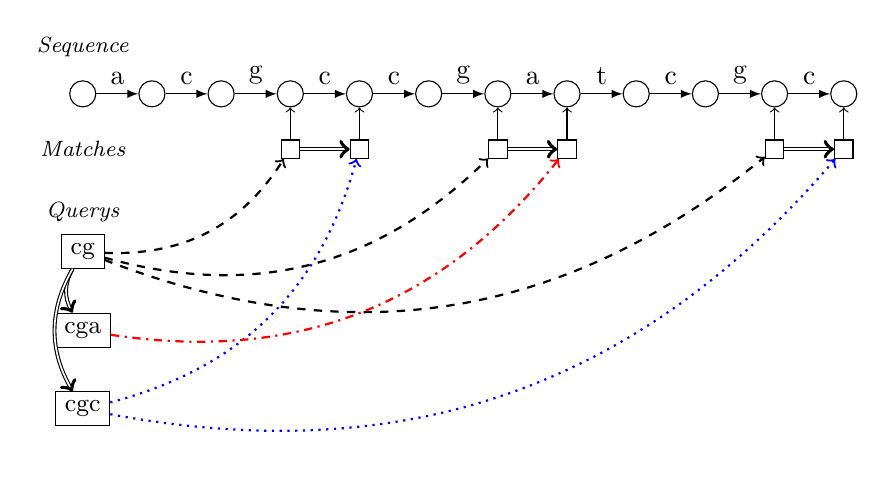
\begin{tikzpicture}[auto]
	\tikzstyle{state} = [ draw, circle, thin, node distance = 2.5em, font={\small}];
	\tikzstyle{query} = [ draw, rectangle, thin, node distance = 2.5em, font={\small}];
	\tikzstyle{info} = [font={\itshape\footnotesize}]
	\tikzstyle{point}  = [ ->, thin, font={\small}];
	\tikzstyle{extend} = [ ->, double, font={\small}];
	\tikzstyle{trace} = [ ->, thick, dashed, bend right, font={\small} ];

	\def \seq {x,a,c,g,c,c,g,a,t,c,g,c}

	\foreach \x [count=\xi] in \seq {
		\ifnum 1 < \xi
			\pgfmathparse{int(\xi-1)}
			\let \li \pgfmathresult
			\node[state, right of=\li] (\xi) {};
			\draw[->, >=latex] (\li) to node{\x} (\xi);
		\else
			\node[state] (\xi) {};
		\fi
	}

	\node[info] at (0,0.6) {Sequence};
	\node[info] at (0,-0.7) {Matches};
	\node[info] at (0,-1.5) {Querys};

	\node[query](cg)  at (0,-2) {cg};
	\node[query](cga) at (0,-3) {cga};
	\node[query](cgc) at (0,-4) {cgc};

	\tikzstyle{tracecg} = [ ->, thick, dashed, bend right, color=black ];
	\tikzstyle{tracecga} = [ ->, thick, dashdotted, bend right, color=red ];
	\tikzstyle{tracecgc} = [ ->, thick, dotted, bend right, color=blue ];

	\draw[extend, bend right] (cg) to (cga);
	\draw[extend, bend right] (cg) to (cgc);

	\foreach \xi/\xv in {4/cg,7/cg,11/cg} {
		\node[draw, below of=\xi, node distance=2em] (p\xi) {};
		\draw[point] (p\xi) to (\xi);
		\draw[trace\xv] (\xv) to (p\xi);
	}

	\foreach \xi/\xv in {5/cgc,8/cga,12/cgc} {
		\node[draw, below of=\xi, node distance=2em] (p\xi) {};
		\draw[point] (p\xi) to (\xi);
		\draw[trace\xv] (\xv) to (p\xi);
	}

	\foreach \xi/\yi in {4/5,7/8,11/12} {
		\draw[extend] (p\xi) to (p\yi);
	}
\end{tikzpicture}

\end{figure}

Initially we have matches only for query $CG$. Then by taking
the \emph{next} token from the sequence we can build up
querys $CGA$ and $CGC$.

\subsection{Groups}

One common addition in a pattern language is capturing a group
of tokens. For example we can use $X = [AC]$ to denote both tokens $A, T$. 
By adding where either one transitions we can capture such groups in 
the extension process.

\begin{figure}[H]
	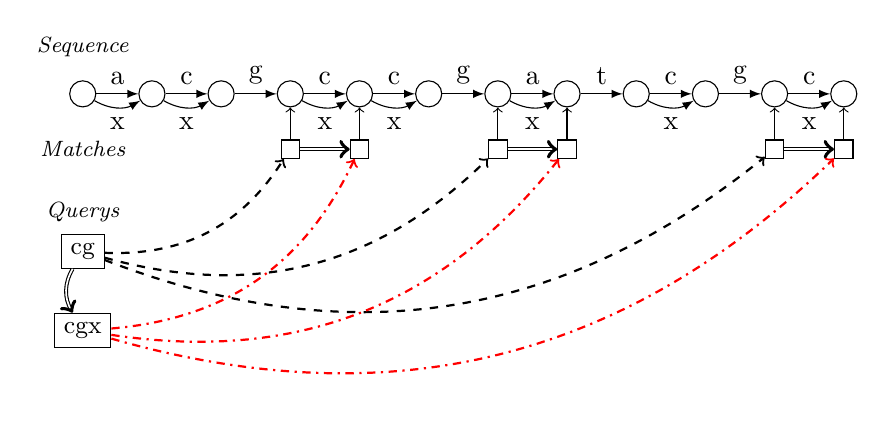
\begin{tikzpicture}[auto]
	\tikzstyle{state} = [ draw, circle, thin, node distance = 2.5em, font={\small}];
	\tikzstyle{query} = [ draw, rectangle, thin, node distance = 2.5em, font={\small}];
	\tikzstyle{info} = [font={\itshape\footnotesize}]
	\tikzstyle{point}  = [ ->, thin, font={\small}];
	\tikzstyle{extend} = [ ->, double, font={\small}];
	\tikzstyle{trace} = [ ->, thick, dashed, bend right, font={\small} ];

	\def \seq {x,a,c,g,c,c,g,a,t,c,g,c}

	\foreach \x [count=\xi] in \seq {
		\ifnum 1 < \xi
			\pgfmathparse{int(\xi-1)}
			\let \li \pgfmathresult
			\node[state, right of=\li] (\xi) {};
			\draw[->, >=latex] (\li) to node{\x} (\xi);
		\else
			\node[state] (\xi) {};
		\fi
	}

	\tikzstyle{exstate} = [ ->, bend right, >=latex];
	\foreach \xi/\yi in {1/2,2/3,4/5,5/6,7/8,9/10,11/12} {
		\draw[exstate] (\xi) to node[below]{x} (\yi);
	}


	\node[info] at (0,0.6) {Sequence};
	\node[info] at (0,-0.7) {Matches};
	\node[info] at (0,-1.5) {Querys};

	\node[query](cg)  at (0,-2) {cg};
	\node[query](cgx) at (0,-3) {cgx};

	\tikzstyle{tracecg} = [ ->, thick, dashed, bend right, color=black ];
	\tikzstyle{tracecgx} = [ ->, thick, dashdotted, bend right, color=red ];

	\draw[extend, bend right] (cg) to (cgx);

	\foreach \xi/\xv in {4/cg,7/cg,11/cg} {
		\node[draw, below of=\xi, node distance=2em] (p\xi) {};
		\draw[point] (p\xi) to (\xi);
		\draw[trace\xv] (\xv) to (p\xi);
	}

	\foreach \xi/\xv in {5/cgx,8/cgx,12/cgx} {
		\node[draw, below of=\xi, node distance=2em] (p\xi) {};
		\draw[point] (p\xi) to (\xi);
		\draw[trace\xv] (\xv) to (p\xi);
	}

	\foreach \xi/\yi in {4/5,7/8,11/12} {
		\draw[extend] (p\xi) to (p\yi);
	}
\end{tikzpicture}

\end{figure}

We shall omit the extension examples since the following of corresponding 
edges is trivial and anologous to previous examples.

\subsection{Star}

Another possible extension is the \emph{dot-star} or more simply capturing
a run of elements. Here we just show the expanded sequence with $*$ symbol.

\begin{figure}[H]
	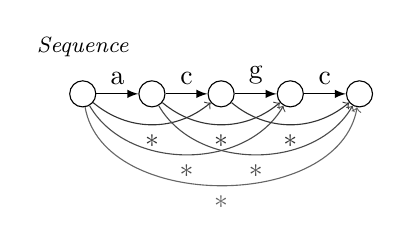
\begin{tikzpicture}[auto]
	\tikzstyle{state} = [ draw, circle, thin, node distance = 2.5em, font={\small}];
	\tikzstyle{query} = [ draw, rectangle, thin, node distance = 2.5em, font={\small}];
	\tikzstyle{info} = [font={\itshape\footnotesize}]
	\tikzstyle{point}  = [ ->, thin, font={\small}];
	\tikzstyle{extend} = [ ->, double, font={\small}];
	\tikzstyle{trace} = [ ->, thick, dashed, bend right, font={\small} ];

	\def \seq {x,a,c,g,c}

	\foreach \x [count=\xi] in \seq {
		\ifnum 1 < \xi
			\pgfmathparse{int(\xi-1)}
			\let \li \pgfmathresult
			\node[state, right of=\li] (\xi) {};
			\draw[->, >=latex] (\li) to node{\x} (\xi);
		\else
			\node[state] (\xi) {};
		\fi
	}

	\node[info] at (0,0.6) {Sequence};

	\tikzstyle{star} = [ ->, bend right, thin, color=black ];

	\foreach \xi in {1,...,3} {
		\pgfmathparse{int(\xi+2)}
		\let \xinext \pgfmathresult
		\foreach \yi in {\xinext,...,5} {
			\pgfmathparse{int(\yi - \xi)}
			\let \df \pgfmathresult
			\pgfmathparse{-\df*20}
			\let \out \pgfmathresult
			\pgfmathparse{int(180 - \out)}
			\let \in \pgfmathresult
			\pgfmathparse{int(100-\df*10)}
			\let \shade \pgfmathresult
			\draw[star, out=\out, in=\in, color=black!\shade] (\xi) to node[below]{$*$} (\yi);
		}
	}

\end{tikzpicture}

\end{figure}

Here we immediately notice how the complexity increases by introducing 
pattern token. Since this is a intermediary step isn't necessary we can 
instead extend with $*Y$, where $Y$ is some other token. This means we 
avoid this single large query and have multiple smaller queries.

\begin{figure}[H]
	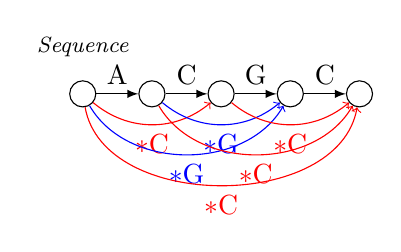
\begin{tikzpicture}[auto]
	\tikzstyle{state} = [ draw, circle, thin, node distance = 2.5em, font={\small}];
	\tikzstyle{query} = [ draw, rectangle, thin, node distance = 2.5em, font={\small}];
	\tikzstyle{info} = [font={\itshape\footnotesize}]
	\tikzstyle{point}  = [ ->, thin, font={\small}];
	\tikzstyle{extend} = [ ->, double, font={\small}];
	\tikzstyle{trace} = [ ->, thick, dashed, bend right, font={\small} ];


	\def \seq {X,A,C,G,C}

	\foreach \x [count=\xi] in \seq {
		\ifnum 1 < \xi
			\pgfmathparse{int(\xi-1)}
			\let \li \pgfmathresult
			\node[state, right of=\li] (\xi) {};
			\draw[->, >=latex] (\li) to node{\x} (\xi);
		\else
			\node[state] (\xi) {};
		\fi
	}

	\node[info] at (0,0.6) {Sequence};

	\tikzstyle{starC} = [ ->, bend right, thin, color=red ];
    \tikzstyle{starG} = [ ->, bend right, thin, color=blue ];

	\foreach \xi in {1,...,3} {
        \foreach \y [count=\yi] in \seq {
            \ifnumless{\xi+1}{\yi}{
                \pgfmathparse{int(\yi - \xi)}
                \let \df \pgfmathresult
                \pgfmathparse{-\df*20}
                \let \out \pgfmathresult
                \pgfmathparse{int(180 - \out)}
                \let \in \pgfmathresult

                \let \pat \seq[3]
                \draw[star\y, out=\out, in=\in] (\xi) to node[below]{$*$\y} (\yi);
            }
        }
	}

\end{tikzpicture}

\end{figure}

We can also limit the length of the run.

\begin{figure}[H]
	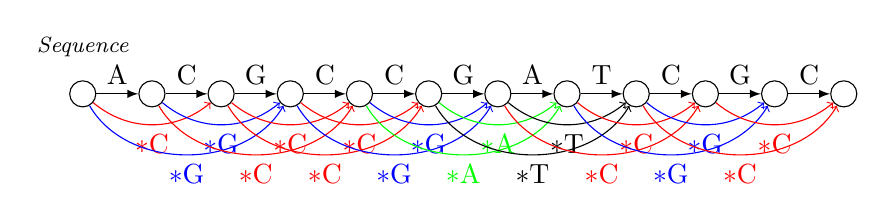
\begin{tikzpicture}[auto]
	\tikzstyle{state} = [ draw, circle, thin, node distance = 2.5em, font={\small}];
	\tikzstyle{query} = [ draw, rectangle, thin, node distance = 2.5em, font={\small}];
	\tikzstyle{info} = [font={\itshape\footnotesize}]
	\tikzstyle{point}  = [ ->, thin, font={\small}];
	\tikzstyle{extend} = [ ->, double, font={\small}];
	\tikzstyle{trace} = [ ->, thick, dashed, bend right, font={\small} ];


	\def \seq {X,A,C,G,C,C,G,A,T,C,G,C}

	\foreach \x [count=\xi] in \seq {
		\ifnum 1 < \xi
			\pgfmathparse{int(\xi-1)}
			\let \li \pgfmathresult
			\node[state, right of=\li] (\xi) {};
			\draw[->, >=latex] (\li) to node{\x} (\xi);
		\else
			\node[state] (\xi) {};
		\fi
	}

	\node[info] at (0,0.6) {Sequence};

	\tikzstyle{starC} = [ ->, bend right, thin, color=red ];
    \tikzstyle{starG} = [ ->, bend right, thin, color=blue ];
    \tikzstyle{starA} = [ ->, bend right, thin, color=green ];
    \tikzstyle{starT} = [ ->, bend right, thin, color=black ];

	\foreach \x [count=\xi] in \seq {
        \foreach \y [count=\yi] in \seq {
        	\pgfmathparse{int(\yi - \xi)}
            \let \df \pgfmathresult

            \ifnumcomp{1}{<}{\df}{
               	\ifnumcomp{\df}{<}{4}{
                	\pgfmathparse{-\df*20}
	                \let \out \pgfmathresult
	                \pgfmathparse{int(180 - \out)}
	                \let \in \pgfmathresult

	                \let \pat \seq[3]
	                \draw[star\y, out=\out, in=\in] (\xi) to node[below]{$*$\y} (\yi);
                }{}
            }{}
        }
	}

\end{tikzpicture}

\end{figure}

Here we have limited the run length to be either 2 or 3.

\subsection{Optimizations}

We can further optimize \emph{group next} by inferring the positions from 
simple \emph{sequence next}. We can see that the positions of a group 
extension is the same as the union of positions by the group tokens.

If we have a group token $\gamma$ that contains $tokens(\gamma)$ then 
the \emph{matches} for such group is $$matches(p\gamma, D) = \bigcup_{t \in tokens(\gamma)} matches(pt, D) $$
    \chapter{Parallelization}
\label{c:parallelization}

Here we discuss different ways of reifying the algorithm to support parallelism. There are several ways of making a program parallel. Using parallelization means that there is a need for some communication and synchronization to make the processes reach the final result. So, it is useful to find as many possible parallelizations as possible, but it is not wise to use all of them.

\section{Process}

This is the main process of the algorithm as described by data flow diagram.\cite{Kahn74,Lee95} Circles denote processes and unfinished rectangles denote data stores.

\begin{figure}[H]
	\scalebox{0.8}{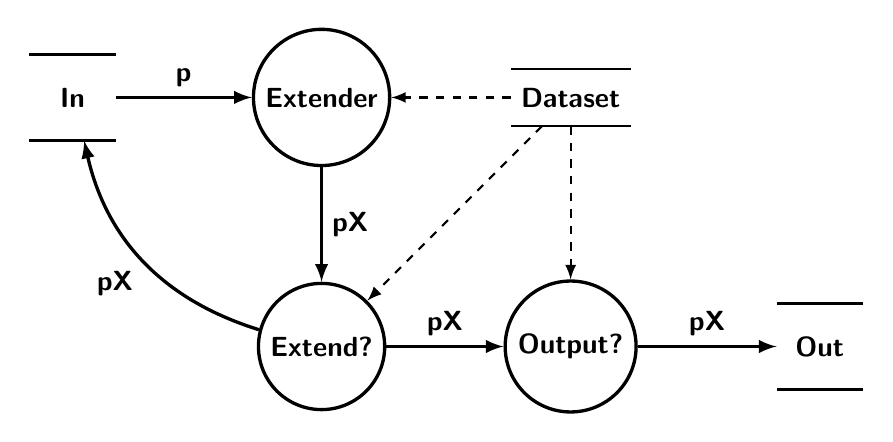
\begin{tikzpicture}[auto]
	\node[pool] (in) {In};
	\node[process, right of=in] (ext) {Extender};
	\node[process, below of=ext] (extable) {Extend?};

	\node[process, right of=extable] (outable) {Output?};
	\node[pool, right of=outable] (out) {Out};

	\node[dataset, right of=ext] (dataset) {Dataset};

	\draw[needs] (dataset) to (ext);
	\draw[needs] (dataset) to (outable);
	\draw[needs] (dataset) to (extable);

	\draw[chan] (in) to node{p} (ext);
	\draw[chan] (ext) to node{pX} (extable);
	\draw[chan]	(extable) to node{pX} (outable);
	\draw[chan, bend left] (extable) to node{pX} (in);
	\draw[chan] (outable) to node{pX} (out);
\end{tikzpicture}
}
\end{figure}

We can see that the different query extension processes do not share a dependency, except the dataset. Dataset itself is read-only in a given process, which means that we can use multiple extender processes. The same applies for extendable and output filter.

\begin{figure}[H]
  \scalebox{0.8}{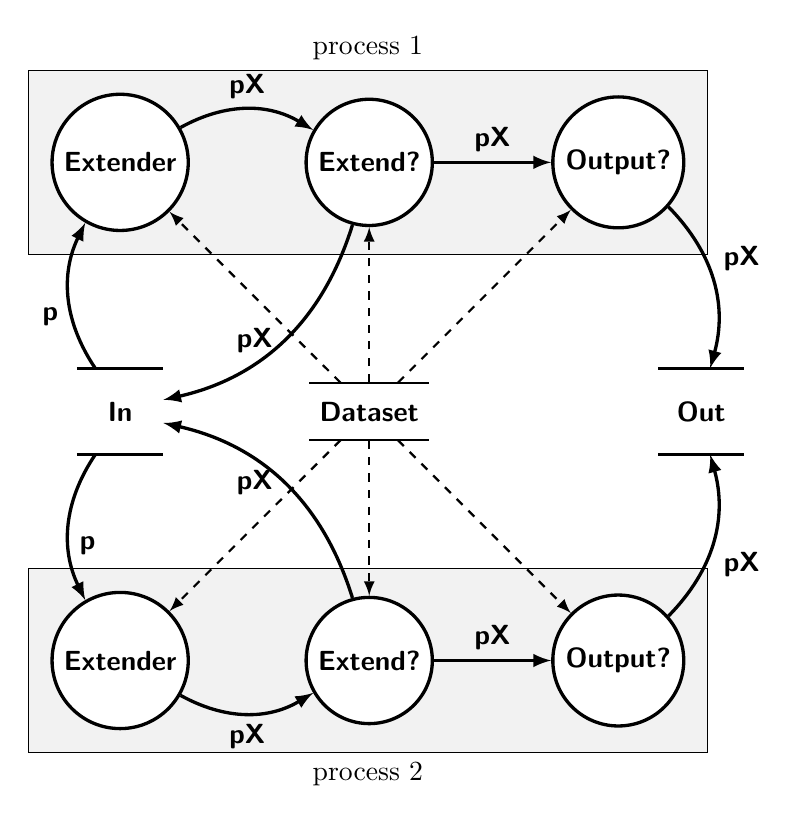
\begin{tikzpicture}[auto]
	\node[pool] (in) {In};

	% upper part	
	\begin{scope}[wrap={label={above:process 1}, inner sep=2ex,fill=black!5}]
		\node[process, above of=in] (ext1) {Extender};
		\node[process, right of=ext1] (extable1) {Extend?};
		\node[process, right of=extable1] (outable1) {Output?};
	\end{scope}

	% lower part
	\begin{scope}[wrap={label={below:process 2}, inner sep=2ex,fill=black!5}]
		\node[process, below of=in] (ext2) {Extender};
		\node[process, right of=ext2] (extable2) {Extend?};
		\node[process, right of=extable2] (outable2) {Output?};
	\end{scope}


	\node[dataset, right of=in] (dataset) {Dataset};
	\node[pool, right of=dataset, node distance=12em] (out) {Out};

	\draw[needs] (dataset) to (ext1);
	\draw[needs] (dataset) to (outable1);
	\draw[needs] (dataset) to (extable1);	

	\draw[needs] (dataset) to (ext2);
	\draw[needs] (dataset) to (outable2);
	\draw[needs] (dataset) to (extable2);

	% upper part flow
	\draw[chan, bend left] (in) to node{p} (ext1);
	\draw[chan, bend left] (ext1) to node[above]{pX} (extable1);
	\draw[chan, bend left] (extable1) to node[left]{pX} (in);
	\draw[chan]	(extable1) to node{pX} (outable1);	
	\draw[chan, bend left] (outable1) to node{pX} (out);

	% lower part flow
	\draw[chan, bend right] (in) to node{p} (ext2);
	\draw[chan, bend right] (ext2) to node[below]{pX} (extable2);
	\draw[chan, bend right] (extable2) to node[left]{pX} (in);
	\draw[chan]	(extable2) to node{pX} (outable2);
	\draw[chan, bend right] (outable2) to node[below right]{pX} (out);	
\end{tikzpicture}
}
\end{figure}

We can add more processes in a similar fashion without affecting the end result. However, such concurrency will introduce a source of indeterminism.

\section{Extending}

The extender can be parallelized via map and reduce concepts\cite{MapReduce,SteeleFold}. The extender was based on two concepts: finding the \emph{next} positions from a previous pattern position, and then grouping those positions together to find the next queries.

The next positions can easily be found from the previous position via mapping by using the \emph{next} function of the dataset. The grouping requires some extra attention - the grouping is a reduction into a map by a key with joining.

Creating a pseudo-code representation of such function compositions would be very difficult and it would require a lot of new syntax. Therefore, we present this idea in Clojure\cite{clojure} which should be readable to people who know lisp. We use the reducers library to show how the extension can be implemented.

\begin{algorithm}[H]
	\caption{Parallel extender}
\begin{lstlisting}[language=Lisp]
(require '[clojure.core.reducers :as r])

; fold-join based grouping function
(defn group-map-by [g f coll]
  (r/fold 
   (r/monoid (partial merge-with into) (constantly {}))
   (fn [ret x]
     (let [k (g x)]
       (assoc ret k (conj (get ret k []) (f x)))))
   coll))

(defn extend [dataset query]
   (let [ steps   (r/mapcat #(walk dataset %) (:positions query))
          grouped (group-map-by :token :position steps)]
        (r/map #(child-query q %) grouped))))
\end{lstlisting}
\end{algorithm}

Such an approach may not give much improvement on desktop CPUs, since we already can process multiple queries at the same time. This parallelization could be beneficial for highly parallel processors such as GPGPUs or FPGAs.

\section{Distributed processes}

Since the dataset and the process memory consumption can get quite large it would also be beneficial to partition the dataset between multiple machines. This can also help on a single machine, since we can interlace running the different processes and store the non-running process in non-volatile memory.

The extension results for a given query stay inside the sequence, which means that we can partition the dataset by assigning sequences to separate datasets.

The whole dataset is required only for filtering queries, since simplest operations ("counting matches in dataset") require full knowledge of all matches over the dataset. We can calculate partial results and let the filters communicate the results. This could also be done in a separate process instead of using direct communication.

\begin{figure}[H]
	\scalebox{0.8}{\begin{tikzpicture}[auto]
	\node[process] (extable) {Extend?};

	% lower part
	\begin{scope}[wrap={label={below:process 2}, inner sep=2ex,fill=black!5}]
		\node[pool, below right of=extable] (in1) {In};
		\node[dataset, right of=in1] (data1) {Dataset 2};
		\node[process, below left of=data1, xshift=2em] (ext1) {Extender};
		\node[process, left of=ext1] (extable1) {Extend?};
		\node[process, right of=ext1] (outable1) {Output?};
	\end{scope}

	\begin{scope}[wrap={label={above:process 1}, inner sep=2ex,fill=black!5}]
		\node[pool, above right of=extable] (in2) {In};
		\node[dataset, right of=in2] (data2) {Dataset 1};
		\node[process, above left of=data2, xshift=2em] (ext2) {Extender};
		\node[process, left of=ext2] (extable2) {Extend?};
		\node[process, right of=ext2] (outable2) {Output?};
	\end{scope}

	\node[process, right of=in, xshift=8em] (outable) {Output?};

	\node[pool, right of=outable, node distance=6em] (out1) {Out};
	\node[pool, right of=outable, node distance=6em] (out2) {Out};

	\draw[needs] (data1) to (ext1);
	\draw[needs] (data1) to (outable1);
	\draw[needs] (data1) to (extable1);

	\draw[needs] (data2) to (ext2);
	\draw[needs] (data2) to (outable2);
	\draw[needs] (data2) to (extable2);

	\draw[chan] (outable) to (out1);
	\draw[chan] (outable) to (out2);

	% lower part flow
	\draw[chan, bend left] (in1) to node[left]{p} (ext1);
	\draw[chan]	(ext1) to node{pX} (outable1);
	\draw[chan, bend left] (ext1) to node{pX} (extable1);
	\draw[chan, bend right] (outable1) to node[right]{pX,Z} (outable);

	% upper part flow
	\draw[chan, bend right] (in2) to node{p} (ext2);
	\draw[chan]	(ext2) to node{pX} (outable2);
	\draw[chan, bend right] (ext2) to node[above]{pX} (extable2);
	\draw[chan, bend left] (outable2) to node{pX,Z} (outable);

	% sync extable
	\draw[chan, bend left] (extable1) to node[draw, diamond](ok1){pX} (in1);
	\draw[chan, bend left] (extable1) to node{Z} (extable);
	\draw[chan] (extable) to node{ok?} (ok1);

	\draw[chan, bend right] (extable2) to node[left, draw, diamond](ok2){pX} (in2);
	\draw[chan, bend right] (extable2) to node[left]{Z} (extable);
	\draw[chan] (extable) to node{ok?} (ok2);
\end{tikzpicture}
}
\end{figure}

\begin{exmp}
For example, to see whether some query is over some count limit, we first count matches in the partial datasets. Then the processes exchange the partial results and add these results together locally. Depending on the local result and filter configuration whether to discard or keep the query.
\end{exmp}

Such distribution could be used to separate the process into more manageable chunks, but, at the same time, it adds significant communication overhead.
    \chapter{Implementation}

Here we discuss a practical implementation, \emph{spexs2}, for
pattern discovery in sequences.

The actual implementation may need to diverge from the abstract
definition for several reasons; mainly practicality, simplicity and
performance. Many of the operations can be optimized for some 
particular type of datasets and configuration.

In this chapter we will discuss parts of program that the author
considers non-trivial in it's design decisions. Information about 
the full source code is in the Appendix B and C.

\section{Architecture}

The main criteria for designing program have been described in D. Parnas
paper On the Decomposition of Programs. It suggests decomposing into
isolated units and parts that are likely to change together. \cite{Parnas72}

We chose the following decomposition:

\begin{description}
	\item[Configuration] structure for holding the configuration data
	\item[Setup] based on the configuration initializes data-structures and functions for the algorithm
	\item[Reader] reads in the data from files
	\item[Database] a collection of datasets
	\item[Algorithm] the SPEXS2 algorithm
		\item[Pattern] represents a pattern
		\item[Query] stores the pattern with database and pattern
		\item[Set] stores matching positions
		\item[Pool] stores queries
		\item[Extender] drives algorithms extending step
		\item[Feature] computes a value from the Query
		\item[Filter] filters some queries
	\item[Printer] prints the result queries
	\item[Debugging] utilities for the program
\end{description}

It is a trivial decomposition for the algorithm part, since a lot of is derived 
directly from the algorithm definition.

The main criteria was to decompose things based on their behavior, whether there
is a commonality between them or whether they change independently from the other
parts.

\section{Configuration}

One problem with flexible algorithms is that they a lot of ways to be run.
This often would need having tens or hundereds of program flags.
To avoid this problem we decided to use a json file for the program
configuration.

\todo[inline]{Short example of a configuration file.}

To properly represent configuration in a static language we
marshal this file directly to the data-structure. This means we can be
less worried about parsing when setting up our algorithm.

The problem with only using a json file is that when running from
command line it may be more comfortable using flags. To solve this problem
we added replacement strings into the json files that can be given in as
a program argument.

\begin{verbatim}
	"Datasets" : {
		"fore" : { "File" : "$inp$"
	...
\end{verbatim}

When using spexs2 --conf conf.json input=filename the input will be
replaced by filename. Also there is optional default value if one wasn't given.

\section{Setup and Database}

Setup consumes the configuration and based on the values initializes pools; 
creates and combines features and filters; reads in the data; and creates
the printer.

\todo[inline]{Database}

\section{Reader and Printer}

One problem with data is that it comes in many different forms. For example reading in 
words and single letters requires different behaviors.

One thing that may be helpful is supporting different binary formats.

\section{Sets}

Since we need a collection how to store the matching positions it suggests
the need for a set datatype.

If we have predictable distribution we can pack the sets better. 

Although such optimizations can be avoided, if during storing pools the
sets are packed using some compression algorithm.

\section{Pools}

There can be different performance characteristics when using a particular implementation. 
Most importantly to support parallelism they should be ideally lock-free, but we can use locked version as well.

For the pools we have several choices: lifo, fifo or priority.

If we use a fifo queue as the in pool the algorithm does a breadth first search of patterns.
This can be problematic since we would need a lot of memory to hold all the patterns in memory.

A lifo queue for in pool is a more reasonable choice for memory problems since we need to hold less patterns in memory.

A priority queue suits for the out pool since we can easily then use some feature to sort 
the queue and choose only a limited amount. A lock-free priority queue would be preferred
but it has many details to work correctly. \todo{link to lock-free queues}

One simple solution to make priority queue concurrent is to use mutexes when storing or
retrieving values. This would mean that many processes can get locked.

We can use some knowledge about the priority-queue behavior. We know that it usually
has limited-size and the amount of patterns suitable for putting into the output
queue is several magnitudes larger; this means most of the queries put into
the result queue are discarded. 

We know that if the query is worse than the worst in the priority queue, it can
be discarded immediately without doing push/pop. If we allow for that check
to fail once in a while - we can make it mostly lock-free.

\begin{verbatim}
	worst := current-worst
	if worst > new-query {
		exit
	}

	mutex.lock
	pqueue.push(new-query)
	current-worst = pqueue.pop()
	mutex.unlock
\end{verbatim}

Although the worst may already have changed after line 1, the algorithm still only keeps the best results.

\section{Features and Filters}

One problem is that the amount of possible filters it's useful to construct them from some other features. 
Or if we wish to use multiple filters we can combine them.

We can use these features to find out something about the query.
They each feature is defined as:

\begin{verbatim}
type Feature func(q *Query) (float64, string)
\end{verbatim}

Most of features are in $\Re$, but for some there
is some extended information that we may wish to know - hence
the need for additional string value. One of the simplest
is Pattern representation.

Also many of the features are defined in terms of multiple datasets.
We can use a closure to easily define a more generic feature.

Example:

\begin{verbatim}
func Matches(dataset []int) Feature {
	return func(q *Query) (float64, string) {
		matches := countf(q.Pos, dataset)
		return matches, ""
	}
}
\end{verbatim}

Here the Matches function creates a feature function defined
for dataset.

We can use the name in the configuration file as "Matches(fore)".

If a feature returns a floating point value we can easily turn that
into a filter by specifying a minimum or/and maximum value.

For example to give a lower and higher limits to some feature:

\begin{verbatim}
func featureFilter(feature Feature, min float64, max float64) Filter {
	return func(q *Query) bool {
		v, _ := feature(q)
		return (min <= v) && (v <= max)
	}
}
\end{verbatim}

Of course there are some filters that cannot be defined by features hence
there is still possibility to make separate filters. Such as disallowing
star symbol in the beginning of the pattern.

\section{Debugging}

Debugging is a important part of development process hence the need for 
more information how the algorithm is working.

Often this is resolved by adding some debug statments:

\begin{verbatim}
for i := 0; i < 100; i += 1{
	printf("picking")
	a := pick()
	printf("picked %v", a)

	printf("picking")
	b := pick()
	printf("picked %v", b)
	
	out.put(a + b)
}
\end{verbatim}

This can be harmful to the readability of the code. To fix this debugging problem we use closures.

\begin{verbatim}
type PickFunc func()Thing
func debuggable(fn PickFunc) PickFunc {
	return func() Thing {
		printf("start picking")
		p := fn()
		printf("picked %v" p)
		return p
	}
}

pick = debuggable(pick)
for i := 0; i < 100; i += 1{
	a := pick()
	b := pick()
	out.put(a + b)
}
\end{verbatim}

As we can see the algorithm implementation is much more readable and 
we can inject different debugging statements without actually changing the algorithm.

Also we can now change the ways how to add debug info. One of would 
be a full stepwise debugger.

\begin{verbatim}
func debuggable(fn PickFunc) PickFunc {
	return func() Thing {
		mutex.lock()
		p := fn()
		while not continue
			interact with user
		mutex.unlock()
		return p
	}
}
\end{verbatim}
    \chapter{Applications and experimental results}

\WIP

\section{Examples}

Here we show examples for the program:

\subsection{DNA sequences}

\todo[inline]{make an example}

\subsection{Protein sequences}

\todo[inline]{make an example}

\subsection{Text mining}

\todo[inline]{make an example}

\subsection{Code mining}

\todo[inline]{make an example}

\section{Performance}

\todo[inline]{make an example}
    \chapter{Conclusions}
\label{c:conclusions}

In this thesis we analyzed how to develop a parallel pattern discovery algorithm. We showed how we can take an already existing algorithm and parallelize it by generalizing, decomposing and then reifying. Finding the general idea of the algorithm can simplify the algorithm and provide more intuitive ways of interpreting it. Decomposing the algorithm allows us to talk about separate parts of the algorithm and modify them without affecting the general idea of the algorithm. If we have an abstract algorithm we can substitute those parts with parallel structures and algorithms.

As a practical part we implemented a parallelized algorithm based on \emph{spexs}\cite{spexs}. We discussed several problems of implementing an algorithm and interesting approaches to these problems. The program has been designed to be easily extendable for different inputs, filters and interestingness criteria. We discussed different possible uses for the implementation and analyzed the performance gained from parallelization.

Approaches suggested in this thesis could be used to generalize and parallelize other algorithms. Finding generic algorithms can be an easy way of discovering new optimizations, new algorithms and new potential applications for algorithms. If these generalizations can be implemented practically, we make the implementation easily extendable and also usable for a wider range of problems.

\chapter*{Paralleelne Mustriotsing}
\label{c:kokkuvote}
\addcontentsline{toc}{chapter}{\numberline{}Kokkuvõte}

\begin{flushleft}
  {\large Egon Elbre } \\[2mm]
  {\large Magistritöö } \\[6mm]
\end{flushleft}

Selles töös uurisime, kuidas arendada paralleelset mustrituvastus algoritmi. Näitasime, kuidas võtta olemasolev algoritm ning paralleliseerida see üldistades, liigendades ja reifitseerides. Algoritmi üldistamine võib tuua esile intuitiivse algoritmi interpretatsiooni. Liigendatud algoritmis on võimalik iga osa eraldi käsitleda algoritmi tulemust muutmata. Asendades iga osa paralleelsete struktuuride ja algoritmidega, saamegi paralleelse algoritmi.

Praktilise osana implementeerisime paralleliseeritud algoritmi \emph{spexs2} võttes aluseks algoritmi SPEXS\cite{spexs}. Seejärel arutlesime erinevate probleemide üle, mis tekkisid algoritmi implementeerimisel. \emph{spexs2}-te on võimalik laiendada erinevate sisendandmetega, otsingufiltritega ja huvitavuskriteeriumitega. Pakkusime välja erinevaid algoritmi kasutusvõimalusi ning analüüsisime paralleliseerimise tulemusel saavutatud kiirusevõitu.

Selles töös tutvustatud ideid saab kasutada algoritmide üldistamisel ja paralleliseerimisel. Algoritmi üldistamisel on võimalik leida uusi viise kuidas algoritmi optimeerida ning avastada uusi algoritme ja leida uusi kasutusvaldkondi sellele algoritmile. Üldistuste implementeerimisel saame programmi, mida on lihtne laiendada ning mida saab kasutada erinevate probleemide lahendamiseks.


    
    \addcontentsline{toc}{chapter}{\numberline{}Bibliography}

    {%\scriptsize
    	\nocite{*}
        \bibliographystyle{ieeetr}
        \bibliography{bibliography}
    }

    \begin{appendix}
        \chapter{spexs2}
\label{add:spexs2}

The program can be found at \url{github.com/egonelbre/spexs}.

Several configurations can be found in the folder \emph{examples}.
It is best to start with an already existing configuration and 
modify it to your needs.

If the running \emph{spexs2 --details} will print
extended help about all the available features, filters, extenders.


        \section{source}

The source code in \emph{src} has the following structure:

\dirtree{%
	.1 src/.
		.2 spexs \DTcomment{algorithm definition}.
			.3 extenders/ \DTcomment{query extenders}.
			.3 features/ \DTcomment{query feature calculators}.
			.3 filters/ \DTcomment{filter implementations}.
			.3 pool/ \DTcomment{different queue implementations}.
			.3 database.go \DTcomment{sequence dataset definition}.
			.3 query.go \DTcomment{query definition}.
			.3 spexs.go \DTcomment{algorithm implementation}.
		.2 spexs2 \DTcomment{command-line utility}.
			.3 conf.go \DTcomment{configuration reader}.
			.3 dataset.go \DTcomment{dataset reader}.
			.3 features.go \DTcomment{parses and creates feature functions}.
			.3 help.go \DTcomment{prints help for the program}.
			.3 printer.go \DTcomment{prints the final output}.
			.3 runtime.go \DTcomment{profiling and live-view setup}.
			.3 setup.go \DTcomment{prepares everything for algorithm}.
			.3 spexs2.go \DTcomment{main-entry point}.
}

There are also additional packages:

\dirtree{%
	.1 src/.
		.2 debugger/ \DTcomment{debugger for concurrent processes}.
		.2 stats/ \DTcomment{statistical functions}.
			.3 binom/ \DTcomment{binomial p-value calculation}.
			.3 hyper/ \DTcomment{hypergeometric p-value calculation}.
		.2 utils/ \DTcomment{additional utility functions}.
		.2 bit/ \DTcomment{functions for bitmanipulation}.
		.2 set/ \DTcomment{set implementations}.
			.3 hash/ \DTcomment{hash table with entry per value}.
			.3 bin/ \DTcomment{hash table with bitvectors}.
			.3 trie/ \DTcomment{2-level hashtable with bitvectors}.
}

For compilation there are two scripts \emph{make.bat} and \emph{make.sh} 
that build the program into bin directory.
        % \chapter{Concise Implementation}
\label{add:epps}

This is a concise implementation of the algorithm for reference.

This part assumes knowledge of \emph{lisp} like languages. 
The code here is presented in Clojure dialect and for an 
introduction on the language see \url{clojure.org/getting_started}.

\missingfigure{write code}
    \end{appendix}
\end{document}